\section{Sampling Random Catalan Objects}%
\label{sec:catalan_objects}
%\todo{Mention that this is imperfect sampling (close impl.)}
%Earlier, we were interested in querying the following random object.
%In a random permutation of $n$ white marbles and $n$ black marbles, how many white marbles are present in the first $k$ positions.
%As we have seen before, \todo{we have?} \cite{huge} gives us a method of sampling from this (hypergeometric) distribution.
%In constructing a generator for the Stochastic Block model, we generalized this by adding more colors (multivariate hypergeometric distribution).
%We also took this to the extreme where all marbles are distinguishable (i.e. a random permutation),
%and saw that this could also be implemented efficiently.
%Now we focus on a more challenging variant of this question with more complicated conditional dependences among the placement of the marbles.
%\todo{Connect with previous part on SBM}
\todo[inline,color=red!80!green!25]{$S_{left}$ etc are too large to compute, but we can approximate teh ratios.}

In the previous Section~\ref{sec:application_sbm} on the Stochastic Block Model, we considered random sequences of colored marbles.
Next, we focus on an important variant of these sequences as Catalan objects, which impose a global constraint on the types of allowable sequences.
Specifically, consider a sequence of $n$ white and $n$ black marbles,
such that every \emph{prefix} of the sequence has at least as many white marbles as black ones.
Our goal will be to support queries to a uniformly random instance of such an object.

\begin{figure}[htbp]
    \centering
    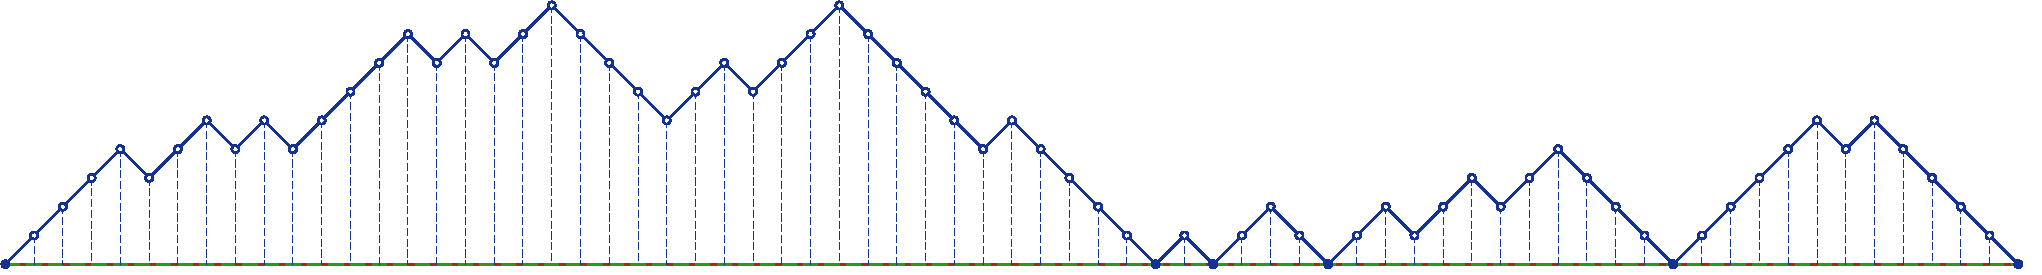
\includegraphics[width=\textwidth]{images/basic_dyck_path.pdf}
    \caption{Simple Dyck path with $n = 35$ up and down steps.}
    \label{fig:basic_dyck}
\end{figure}
One interpretation of Catalan objects is given by Dyck paths (Figure~\ref{fig:basic_dyck}).
A Dyck path is essentially a $2n$ step \emph{balanced} one-dimensional walk with exactly $n$ up and down steps.
In Figure~\ref{fig:basic_dyck}, each step moves one unit along the positive $x$-axis (time) and one unit up or down the positive $y$-axis (position).
The prefix constraint implies that the $y$-coordinate of any point on the walk is $\ge 0$ i.e. the walk never crosses the $x$-axis.
The number of possible Dyck paths (see Theorem~\ref{thm:number_of_dyck_paths}) is the $n^{th}$ Catalan number $C_n=\frac{1}{n+1}\cdot{2n\choose n}$.
Many important combinatorial objects occur in Catalan families of which these are an example.

\textcolor{Maroon}{We will approach the problem of partially sampling Catalan objects through Dyck paths.}
This, in turn, will allow us to sample other random Catalan objects such as rooted trees, and bracketed expressions.
Specifically, we will want to answer the following queries:
\begin{itemize}
    \item \textcolor{Maroon}{\func{Direction}$(i)$: Returns the value of the $i^{th}$ step in the Dyck path (whether the step is up or down).}
    \item \func{Height}$(i)$: Returns the position of the path after $i$ steps.
    \item \func{First-Return}$(i)$: Returns an index $j>i$ such that $\func{Height}(j)=\func{Height}(i)$, and for any other $k$ between $i$ and $j$,
    $\func{Height}(k)$ is strictly greater than $\func{Height}(i)$.
    \textcolor{Maroon}{
    While it may not be clear why this kind of query is important, it will be useful for querying bracketed expressions and random trees.
    We defer this discussion to Section~\ref{sec:bijections_to_other_catalan_objects}.}
\end{itemize}
\textcolor{Maroon}{Since a $\func{Direction}(i)$ query can be simulated using the queries $\func{Height}(i)$ and $\func{Height}(i-1)$,
we will not explicitly discuss the \func{Direction} queries in what follows.}



\subsection{Bijections to other Catalan objects}%
The $\func{Height}$ query is natural for Dyck paths, but the $\func{First-Return}$ query is important in exploring other Catalan objects.
For instance, consider a random well bracketed expression; equivalently an uniform distribution over the Dyck language.
One can construct a trivial bijection between Dyck paths and words in this language
by replacing up and down steps with opening and closing brackets respectively.
The $\func{Height}$ query corresponds to asking for the nesting depth at a certain position in the word,
and $\func{First-Return}(x)$ returns the position of the matched closing bracket for position $x$.

\label{sec:bijections_to_other_catalan_objects}
\begin{figure}[htbp]
    \centering
    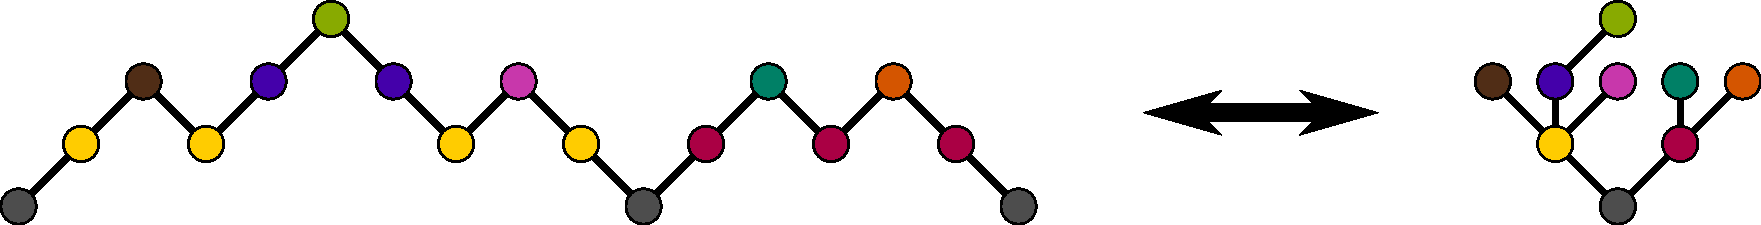
\includegraphics[width=0.9\textwidth]{images/dyck_tree_bijection.pdf}
    \caption{Bijection between Dyck paths and ordered rooted trees.
    For example, successive $\func{First-Return}$ queries on the yellow node would reveal its three children in order from left to right.}
    \label{fig:dyck_tree_bijection}
\end{figure}
There is also a natural bijection between Dyck paths and ordered rooted trees (Figure~\ref{fig:dyck_tree_bijection}),
by considering the Dyck path to be a transcript of a DFS traversal on the tree.
Starting with the root, for each ``up-step'' we move to a new child of the current node, and for each ``down-step'', we backtrack towards the root.
Here, the $\func{Height}$ query returns the depth of a node and the $\func{First-Return}$ query can be used to find the \emph{next child} of a node.
A similar argument shows a bijection to the set of all ordered binary trees.
Moving forwards, we will focus on Dyck paths for the sake of simplicity.

We only consider \func{First-Return}$(x)$ when the step from $x$ to $x+1$ is upwards i.e. when $\func{Height}(x+1) = \func{Height}(x) + 1$.
We can also implement a \func{Reverse-First-Return}$(x)$ query that returns the first return in the reversed Dyck path,
when $\func{Height}(x-1) = \func{Height}(x) + 1$.
As we shall show later (Section~\ref{sec:reverse_first_return_queries}),
this query can also be implemented in a symmetric manner to \func{First-Return}.
Otherwise, the height at $x$ is larger than both the heights at $x-1$ and $x+1$, the $\func{First-Return}$ query has no meaningful value.
This pattern corresponds to consecutive opening and closing braces in bracketed expressions and to a leaf node in rooted trees.
\todo[inline,color=red!80!green!25]{Finish}



\subsection{Catalan Trapezoids and Generalized Dyck Paths}
In order to sample Dyck paths locally, we will need to analyze more general Catalan objects.
Specifically, we consider a sequence of $U$ up-steps and $D$ down-steps,
such that any prefix of the sequence containing $U'$ up and $D'$ down steps satisfies $U'-D' \ge 1-k$.
This means that we start our Dyck path at a height of $k-1$, and we are never allowed to cross below zero (Figure~\ref{fig:complex_dyck}).
Note that the case $k=1$ corresponds to the standard description of Dyck paths, as mentioned previously (Figure~\ref{fig:basic_dyck}).
\begin{figure}[htbp]
    \centering
    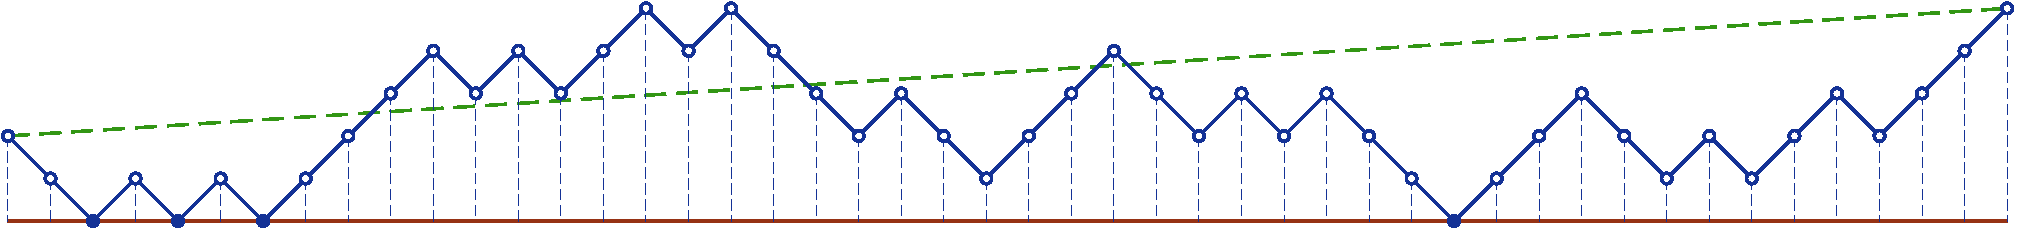
\includegraphics[width=\textwidth]{images/complex_dyck_path.pdf}
    \caption{Generalized Dyck path with $U = 25$, $D = 22$ and $k = 3$.
             Note that the boundary is $k-1 = 2$ units below the starting height.} \label{fig:complex_dyck}
\end{figure}

We will denote the set of such \emph{generalized Dyck paths} as $\mathbb C_k(U,D)$ and the number of paths as $C_k(U,D) = |\mathbb C_k(U,D)|$,
which is an entry in the \textit{Catalan Trapezoid} of order $k$ \cite{trap}.
We also use $\mathsf C_k(U,D)$ to denote the uniform distribution over $\mathbb C_k(n,m)$.
Now, we state a result from \cite{trap} without proof:
\begin{align}
    \label{eq:catalan_trapezoid}
    C_k(U,D)=
    \begin{cases}
    \binom{U+D}{D} &0\le D<k\\
    \binom{U+D}{D} - \binom{U+D}{D-k} &k\le D\le U+k-1\\
    0 &D>U+k-1
    \end{cases}
\end{align}
For $k = 1$ and $n=m$, these represent the vanilla Catalan numbers i.e. $C_n = C_1(n,n)$ (number of simple Dyck paths).
Our goal is to sample from the distribution $\mathsf C_1(n,n)$.

Consider the situation after a sequence of \func{Height} queries to the Dyck path at various locations $\langle x_1, x_2,\cdots, x_m \rangle$,
such that the corresponding heights were sampled to be $ \langle y_1, y_2,\cdots, y_m \rangle$.
These revealed locations partition the path into disjoint \emph{intervals} $[x_i,x_{i+1}]$,
where the heights of the endpoints of each interval have been determined (as $y_i = \func{Height}(x_i)$).
We notice that these intervals can be sampled independently of each other.
Specifically, the path within the interval $[x_i, x_{i+1}]$ will be sampled from $\mathsf C_k(U,D)$,
where $k - 1 = y_i$, $U + D = x_{i+1} - x_i$, and $U-D = y_{i+1} - y_i$.
Moreover, since the heights of the endpoints $y_i$ and $y_{i+1}$ are known, this choice is independent of any samples outside the interval.
Next, in Section~\ref{sec:sampling_the_height}, we will show how one can sample heights within such an interval,
and in Section~\ref{sec:supporting_first_return_queries} we will move on to the more complicated $\func{First-Return}$ queries.

%We also maintain a threshold $\mathcal T = \Theta(\log^4 n)$.
%If a query lands in an interval that has length less than $\mathcal T$, then we brute force sample the entire interval one step at a time.
%Assuming that the probabilities of these events can be approximated efficiently (Lemma~\ref{lem:probability_approximation_oracle},
%this take $\poly(\log n)$ time.
%\todo{Is this necessary?}



\subsection{Sampling the Height}
\label{sec:sampling_the_height}
We implement $\func{Height}(t)$ by showing how to (efficiently) sample the height of the path in the midpoint of an existing interval $[x_i, x_{i+1}]$
(where the heights of the endpoitns are $y_i$ and $y_{i+1}$).
We can then extend this to arbitrary positions by running a binary search on the appropriate interval using the midpoint samples.
If the interval in question has odd length, \textcolor{Maroon}{we sample one step on the boundary}, and proceed with a shortened even length interval.
\begin{figure}[htpb]
    \centering
    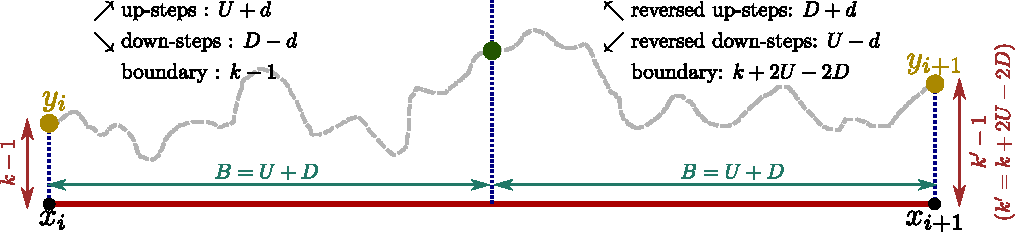
\includegraphics[width=\textwidth]{images/dyck_height_sampling.pdf}
    \caption{The $2B$-interval is split into two equal parts resulting in two separate Dyck problems.
             The green node (center) is the sampled height of the midpoint parameterized by the value of $d$.
             The path considered in both sub-intervals starts at a yellow node (left and right edges) and ends at the green node.
             From this perspective, the path on the right is reversed with up and down steps being swapped.
             A possible path is shown in gray.}
    \label{fig:dyck_height_sampling}
\end{figure}

Our general recursive step is as follows.
We consider an interval of length $2B$ comprising of $2U$ up-steps and $2D$ down-steps where the sum of any prefix cannot be less than $k-1$
i.e. the path within this interval should be sampled from $\mathsf C_k(2U,2D)$.
In order to make the analysis simpler, we have assumed that the number of up and down steps are both even.
The case of sampling according to $\mathsf C_k(2U+1, 2D+1)$ works similarly with slightly different formulae.
Without loss of generality, we assume that $D\le U$; if this were not the case, we could simply flip the interval,
swap the up and down steps, and modify the prefix constraint to $k'=k+2U-2D$ (Figure~\ref{fig:dyck_height_sampling}).
This ensures that the overall path in the interval is non-decreasing in height, which will simpify our analysis.

We determine the height of the path $B = U+D$ steps into the interval at the midpoint (see Figure~\ref{fig:dyck_height_sampling}).
This is equivalent to finding the number of up or down steps that get assigned to the first half of the interval.
We parameterize the possibilities by $d$ and define $p_d$ to be the probability that exactly $U+d$ up-steps and $D-d$ down steps
get assigned to the first half (with the remaining $U-d$ up steps and $D+d$ down steps being assigned to the second half).
\begin{align}
\label{eq:height_sampling_probability}
p_d = \frac{S_{left}(d)\cdot S_{right}(d)}{S_{total}(d)}
\end{align}
Here, $S_{left}(d)$ denotes the number of possible paths in the first half (using $U+d$ up steps)
and $S_{right}(d)$ denotes the number of possible paths in the second half (using $U-d$ up steps).
Note that all of these paths have to respect the $k$-boundary constraint (cannot dip more than $k-1$ units below the starting height), where $k=y_i+1$.
Moving forwards, we will drop the $d$ when referring to the path counts.
We (conceptually) flip the second half of the interval,
such that the corresponding path begins from the end of the $2B$-interval and terminates at the midpoint (Figure~\ref{fig:dyck_height_sampling}).
This results in a different starting point, and the prefix/boundary constraint will also be different.
Hence, we define $k' = k + 2U - 2D$  to represent the new boundary constraint (since the final height of the $2B$-interval is $k'-1$).
Finally, $S_{total}$ is the total number of possible paths in the $2B$ interval.

We will now use the rejection sampling lemma (Lemma~\ref{lem:rejection_sampling}).
An important point to note is that in order to apply this lemma, we must be able to compute the $p_d$ values at least approximately.
For now, we assume that we have access to an oracle that will compute the value for us.
Lemma~\ref{lem:probability_approximation_oracle} in Section~\ref{sec:dyck_appendix} shows how to construct such an oracle.
We also use the following lemma to bound the deviation of the path with high probability.
\begin{restatable}{lemma}{DyckPathDeviationBound}
\label{lem:DyckPathDeviationBound}
Consider a contiguous \emph{sub-path} of a simple Dyck path of length $2n$
where the sub-path is of length $2B$ comprising of $U$ up-steps and $D$ down-steps (with $U + D = 2B$).
Then there exists a constant $c$ such that the quantities $|B-U|$, $|B-D|$, and $|U-D|$
are all $<c\sqrt{B\log n}$ with probability at least $1-1/n^2$ for every possible sub-path.
\end{restatable}
\textcolor{Maroon}{This lemma allows us to ignore potential midpoint heights that cause a deviation greater than $c \sqrt{B\log n}$}.
A proof is presented in Section~\ref{sec:dyck_path_boundaries_and_deviations}.
One implication of Lemma~\ref{lem:DyckPathDeviationBound} is that with high probability,
the correctly sampled value for $d$ will be $\mathcal O(\sqrt{B\log n})$.
In other words, The height of the midpoint takes on one of only  $\mathcal O(\sqrt{B\log n})$ distinct values with high probability.
This immediately suggests a $\tilde{\mathcal O}(\sqrt{B})$ time algorithm for sampling the midpoint height,
by explicitly computing the probabilities of each of these potential heights, and directly sampling from the resulting distribution.
However, we can go further and obtain a $\mathcal O(poly(\log n))$ time algorithm.


\subsubsection{The Simple Case: Far Boundary}%
\label{sec:the_simple_case}
We first consider the case when the boundary constraint is far away from the starting point, i.e. $k$ is large.
The following lemma (proof in Section~\ref{sec:dyck_path_boundaries_and_deviations}) shows that in this case,
we can safely \emph{ignore} the constraint.  Intuitively, this is because the boundary is so far away,
that we do not hit it with high probability even if we choose a random \emph{unconstrained} path.
\begin{restatable}{lemma}{DyckPathIrrelevantBoundary}
\label{lem:dyck_path_irrelevant_boundary}
Given a Dyck path sampling problem of length $B$ with $U$ up and $D$ down steps with a boundary at $k$,
there exists a constant $c$ such that if $k > c \sqrt{B\log n}$, then the distribution of paths sampled without a boundary $\mathsf C_{\infty}(U,D)$
(hypergeometric sampling) is statistically $\mathcal O(1/n^2)$-close in $L_1$ distance to the distribution of Dyck paths $\mathsf C_k(U+D)$.
\end{restatable}
By Lemma~\ref{lem:dyck_path_irrelevant_boundary}, the problem of sampling from $C_k(2U,2D)$
reduces to sampling from the hypergeometric distribution $C_{\infty}(2U,2D)$ when $k>\mathcal{O}(\sqrt{B\log n})$
i.e. the probabilities $p_d$ can be approximated by:
\[
q_d = \frac{{{B}\choose{D-d}}\cdot{{B}\choose{D+d}}}{{{2B}\choose{2D}}}
\]
This problem of sampling from the hypergeometric distribution is implemented using $\mathcal O(poly(\log n))$ resources in \cite{huge}
%in the context of interval summable functions
(see Lemma~\ref{lem:ggn_interval_summable} in Section~\ref{sec:multivariate_hypergeometric_sampling}).
We also used this result earlier in the paper in order to find the community assignments in the Stochastic Block Model
(Section~\ref{sec:application_sbm}).

\subsubsection{The Difficult Case: Intervals Close to Zero}
\label{sec:the_difficult_case}
The difficult case is when $k = \mathcal{O}(\sqrt{B\log n})$,
and the previous approximation due to Lemma~\ref{lem:dyck_path_irrelevant_boundary} no longer works.
In this case, we cannot just ignore the boundary constraint, and instead we have to analyze the true probability distribution given by $p_d$.
We obtain an expression for $p_d$ by substituting the formula for generalized Catalan numbers as follows:
(Equation~\ref{eq:catalan_trapezoid}) into Equation~\ref{eq:height_sampling_probability}.
\begin{align}
    S_{left} = C_k(U+d,D-d)
    &&S_{right} = C_{k'}(U-d,D+d)
    &&S_{total} = C_k(2U,2D)
\end{align}
Since the right interval is flipped in our analysis, this changes the prefix/boundary constraint,
and hence, the expression for $S_{right}$ uses $k' = k+2U-2D$.
This also implies that $k' = \Bo(\sqrt{B\log n})$ (using Lemma~\ref{lem:DyckPathDeviationBound}).
We can now use Equation~\ref{eq:height_sampling_probability} to evaluate the probabilties $p_d = S_{left}\cdot S_{right}/S_{total}$.
Recall that $p_d = S_{left}(d)\cdot S_{right}(d)/S_{total}(d)$, where $S_{left}$ and $S_{right}$ are the number of possible paths
in the left and right half of the interval respectively, when exactly $U+d$ up steps are assigned to the first half.
$S_{total}$ is the total number of possible paths in the interval.

We will invoke the rejection sampling technique (Lemma~\ref{lem:rejection_sampling}), by constructing a different distribution $q_d$
that approximates $p_d$ up to logarithmic factors over the vast majority of its support
(we ignore all $|d|>\Theta(\sqrt{B\log n})$ since the associated probability mass is negligible by Lemma~\ref{lem:DyckPathDeviationBound}).
In order to perform rejection sampling, we also need good approximations of $p_d$,
which is acheved by Lemma~\ref{lem:probability_approximation_oracle} in Section~\ref{sec:computing_probabilities}.
Next, we define an appropriate $q_d$ that approximates $p_d$ and also has an \emph{efficiently computable} $CDF$.
Surprisingly, as in Section~\ref{sec:the_simple_case}, we will be able to use the hypergeometric distribution for $q_d$,
\[
q_d \equiv \frac{{B\choose D-d}\cdot{B\choose D+d}}{{2B\choose 2D}} = \frac{{B\choose D-d}\cdot{B\choose U-d}}{{2B\choose 2D}}
\]
However, the argument for why this $q_d$ is a good approximation to $p_d$ is far less straightforward.

First, we consider the case where $k\cdot k'\le 2U+1$.
In this case, we use loose bounds for $S_{left} < \binom{B}{D-d}$ and $S_{right} < \binom{B}{U-d}$.
The preceding upper bounds hold because $\binom{B}{D-d}$ and $\binom{B}{U-d}$ are the total number of \emph{unconstrained} paths
in the left and right half respectively, and adding the boundary constraint can only reduce the number of paths.
We also prove the following lemma in Section~\ref{sec:dyck_appendix} to bound the value of $S_{right}$.
\begin{restatable}{lemma}{DTotalFarBoundary}
\label{lem:DTotalFarBoundary}
When $kk' > 2U + 1$, $S_{total} > \frac 12\cdot \binom{2B}{2D}$.
\end{restatable}

Combining the three bounds, we conclude that $p_d < \frac 12 q_d$.
Intuitively, in this case the Dyck boundary is far away, and therefore the number of possible paths
is only a constant factor away from the number of unconstrained paths (see Section~\ref{sec:the_simple_case}).
The case where the boundaries are closer (i.e. $k\cdot k' \le 2U+1$) is trickier,
since the individual counts need not be close to the corresponding binomial counts.
However, in this case we can still ensure that the sampling probability is within poly-logarithmic factors of the binomial sampling probability.
We use the following lemmas (proven in Section~\ref{sec:dyck_appendix}).

\begin{restatable}{lemma}{DLeftBound}
\label{lem:DLeftBound}
$S_{left} \le c_1 \frac{ k\cdot\sqrt{\log n}}{\sqrt{B}}\cdot{{B}\choose{D-d}}$ for some constant $c_1$.
\end{restatable}

\begin{restatable}{lemma}{DRightBound}
\label{lem:DRightBound}
$S_{right} \le c_2 \frac{k'\cdot \sqrt{log n}}{\sqrt{B}}\cdot{{B}\choose{U-d}}$ for some constant $c_2$.
\end{restatable}

\begin{restatable}{lemma}{DTotalNearBoundary}
\label{lem:DTotalNearBoundary}
When $kk' \le 2U + 1$, $S_{total} \ge c_3 \frac{k\cdot k'}{B}\cdot{{2B}\choose{2D}}$ for some constant $c_3$.
\end{restatable}

\todo[inline,color=red!80!green!25]{Explain this more?}
We can now put these lemmas together to show that $p_d/q_d \le \Theta(\log n)$ and invoke Lemma~\ref{lem:rejection_sampling} to sample the value of $d$.
This gives us the height of the Dyck path at the midpoint of the two given points.

\begin{theorem}
\label{thm:dyck_midpoint_sampling}
Given an interval $[x_i,x_{i+1}]$ (and the associated endpoint heights $y_i, y_{i+1}$) in a Dyck path of length $2n$,
with the guarantee that no position between $x_i$ and $x_{i+1}$ has been sampled yet,
there is an algorithm that returns the height of the path at the midpoint of $x_i$ and $x_{i+1}$ (or next to the midpoint if $x_{i+1}-x_i$ is odd).
Moreover, this algorithm only uses $\mathcal O(poly(\log n))$ resources.
\end{theorem}
\begin{proof}
If $x_{i+1}-x_i$ is even, we can set $B = (x_{i+1}-x_i)/2$.
Otherwise, we first sample a single step from $x_i$ to $x_i+1$, and then set $B = (x_{i+1}-x_i-1)/2$.
Since there are only two possibilities for a single step, we can explicitly approximate the probabilities, and then sample accordingly.
This allows us to apply the rejection sampling from Lemma~\ref{lem:rejection_sampling}
using $\{ q_d\}$ to obtain samples from $\{ p_d\}$ as defined above.
%Now, if $B > \Theta(\log^2 n)$ we can simply use the rejection sampling procedure described above
%to obtain a $\mathcal O(poly(\log n))$ algorithm.
%Otherwise, we sample each step induividually.
%Since there are only $2B = \Theta(\log^2 n)$ steps, the sampling is still efficient.
\end{proof}

\begin{theorem}
\label{thm:dyck_height_sampling}
There is an algorithm that provides sample access to a Dyck path of length $2n$,
by answering queries of the form \func{Height}$(x)$ with the correctly sampled height of the Dyck path at position $x$
using only $\mathcal O(poly(\log n))$ resources per query.
\end{theorem}
\begin{proof}
The algorithm maintains a successor-predecessor data structure (e.g. Van Emde Boas tree) to store all positions $x$ that have already been sampled.
Each newly sampled position is added to this structure.
Given a query \func{Height}$(x)$, the algorithm first finds the successor and predecessor (say $a$ and $b$) of $x$ among the already queried positions.
This provides us the guarantee required to apply Theorem~\ref{thm:dyck_midpoint_sampling},
which allows us to query the height at the midpoint of $a$ and $b$.
We then binary search by updating either the successor or predecessor of $x$ and repeat until we sample the height of position $x$.
%Once the interval length becomes less than $\Theta(\log^2 n)$,
%we perform the full sampling (as in Theorem~\ref{thm:dyck_midpoint_sampling}) which provides us the height at position $x$.
\end{proof}




\subsection{Supporting ``First Return'' Queries}%
\label{sec:supporting_first_return_queries}
In this section, we show how to implement more complex queries to a Dyck path.
Specifically, we introduce $\func{First-Return}(x)$ to allow the user to query the next time the path returns to \func{Height}$(x)$ (if at all).
The utility of this kind of query can be seen through other random Catalan objects.
For instance, if we consider a random well bracketed expression, $\func{First-Return}(x)$ is the position of the bracket matching the $x^{th}$ one.
If we consider a random rooted tree,
$\func{First-Return}$ corresponds to the next child of a vertex (see Section~\ref{sec:bijections_to_other_catalan_objects}).
An important detail here is that if the first step from $x$ to $x+1$ is an down-step, there is no well defined ``\func{First-Return}''.
In case of trees, this would correspond to a leaf which has no children.

%We will use the following asymptotic formula for \emph{close-to-central} binomial coefficients
%which will allow us the approximate the probabilities in Section~\ref{sec:estimating_the_cdf}.
%\begin{restatable}{lemma}{CentralBinomialCoefficients}
%\label{lem:CentralBinomialCoefficients}
%(From \cite{asymptopia}) If $k = \frac{n \pm c\sqrt n}{2}$ where $c = o(n^{1/6})$,
%we can approximate $\binom{n}{k}$ up to constant factors by the expression $\frac{2^n}{\sqrt n}\cdot \mathlarger e^{-c^2/2}$.
%\end{restatable}

%Recall that we maintain a threshold $\mathcal T = \Theta(\log^4 n)$ such that
%if an un-sampled interval in the Dyck path has length less than $\mathcal T$, then we sample the entire interval using brute force.
%By setting $\mathcal T = \Theta(\log^4 n)$, we see that for intervals with length $B > \mathcal T$,
%the maximum deviations are bounded by $\mathcal O(\sqrt{B\log n}) = \mathcal O(\log^{2.5}n)$ with high probability.
%This means that if we write the deviation as $c\sqrt B$, we see that $c = \mathcal O(\sqrt{\log n})$ which is $o(B^{1/6})$,
%thus satisfying the condition of Lemma~\ref{lem:CentralBinomialCoefficients}.
%\todo{Is this necessary?}


\subsubsection{Maintaining a Boundary Invariant}
\label{sec:maintaining_a_boundary_invariant}
Notice that after performing a set of $\func{Height}$ queries $\langle x_1, x_2,\cdots, x_m \rangle$ to the Dyck path,
many different positions are revealed (possibly in adverserial locations).
This partitions the path into at most $m+1$ disjoint and independent \emph{intervals} with known boundary conditions.
The first step towards finding the $\func{First-Return}$ from position $t$ would be to locate the \emph{interval} where the first return occurs.
Even if we had an efficient technique to filter intervals, we would want to avoid considering all $\Theta(m)$ intervals to find the correct one.
In addition, the fact that a specific interval \emph{does not} contain the first return implies dependencies for all subsequent samples.

We resolve these difficulties by maintaining a new invariant.
Consider all positions whose heights have have already been sampled, either directly as a result of user given $\func{Height}$ queries,
or indirectly due to recursive $\func{Height}$ calls; $\langle x_1, x_2,\cdots, x_m \rangle$ in increasing order i.e. $x_i<x_{i+1}$.
Let the corresponding heights be $ \langle y_1, y_2,\cdots, y_m \rangle$ i.e. $\func{Height}(x_i) = y_i$.
\begin{invariant}
\label{inv:boundary_invariant}
For any interval $[x_i,x_{i+1}]$ where the heights  of the endpoints have been sampled to be $y_i$ and $y_{i+1}$,
and no other position in the interval has yet been sampled,
the section of the Dyck path between positions $x_i$ and $x_{i+1}$ is constrained to lie above $min(y_i, y_{i+1})$.
\end{invariant}
\begin{figure}[htpb]
    \centering
    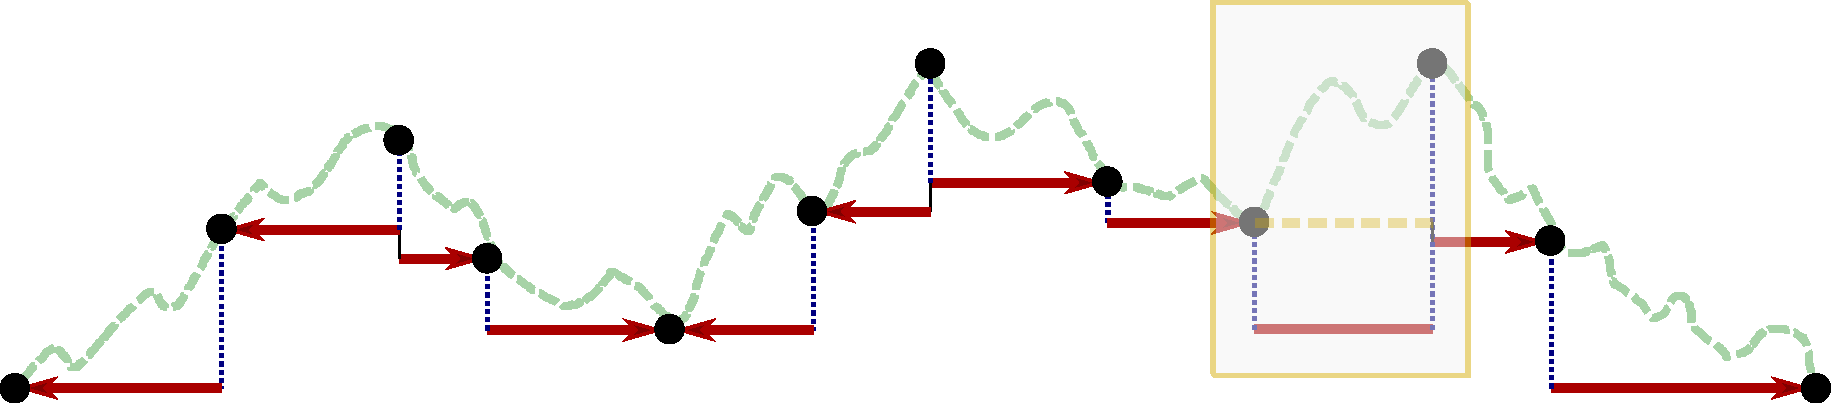
\includegraphics[width=\textwidth]{images/dyck_boundary_invariant.pdf}
    \caption{The set of intervals formed by a set of height samples.
        Each interval also has its own boundary constraint (red).
        Invariant~\ref{inv:boundary_invariant} implies that each boundary must coincide with one of the interval endpoints.
        Note that the only interval which violates the invariant is the third last one (shown in yellow box).}
    \label{fig:dyck_boundary_invariant}
\end{figure}

How can one maintain such an invariant?
After sampling the height of a particular position $x_i$ as $y_i$ (with $x_{i-1} < x_i < x_{i+1}$),
the invariant is potentially broken on either side of $x_i$.
We re-establish the invariant by sampling an additional point on either side.
This proceeds as follows for some violating interval $[x_i, x_{i+1}]$ (example violation in Figure~\ref{fig:dyck_boundary_invariant}):
\begin{enumerate}
    \item \textcolor{Maroon}{Sample} the lowest height $h$ achieved by the walk between $x_i$ and $x_{i+1}$ according to
    the uniform distribution over all possible paths that respect the current boundary constraint
    (see Section~\ref{sec:sampling_the_lowest_achievable_height}).
    \item \textcolor{Maroon}{Sample} an intermediate position $x$ such that $x_i < x < x_{i+1}$ and $\func{Height}(x) = h$
    (see Section~\ref{sec:sampling_first_position_touching_mandatory_boundary}).
\end{enumerate}
The sample $\func{Height}(x)$ results in two sub-intervals $[x_i, x]$ and $[x, x_{i+1}]$.
Since $h = \func{Height}(x)$ has been determined to be the minimum height in the overall range $[x_i, x_{i+1}]$,
the invariant is preserved in the new intervals (see Figure~\ref{fig:dyck_invariant_preserve}).
Lemma~\ref{lem:first_return_interval} in Section~\ref{sec:finding_the_correct_interval}
shows how this invariant can help us efficiently search for the interval containing the first return.
\begin{figure}[htpb]
    \centering
    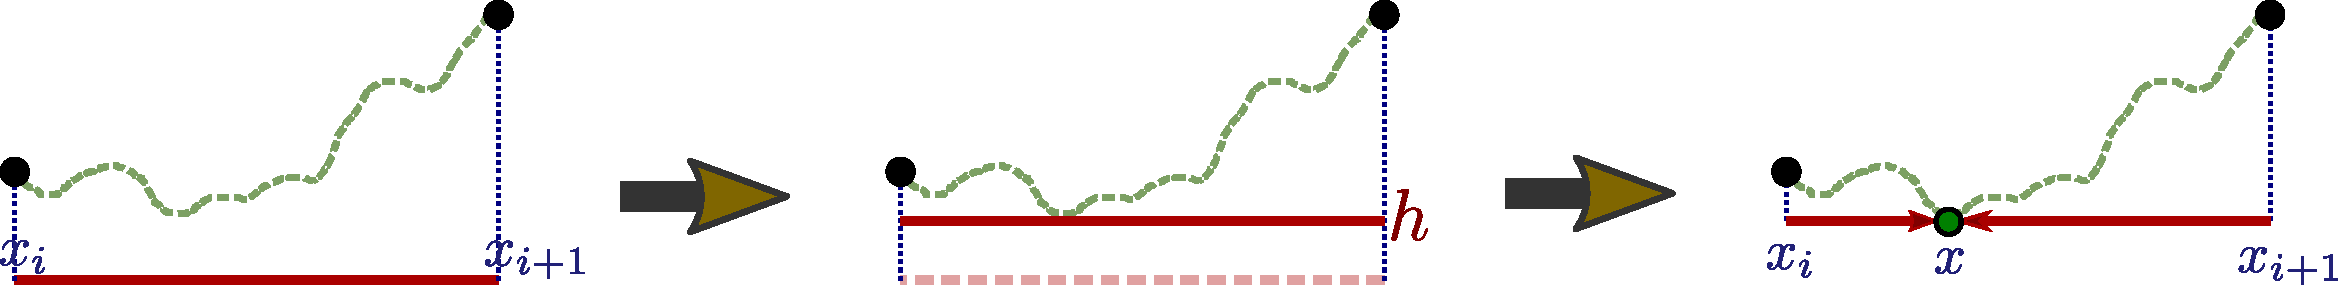
\includegraphics[width=\textwidth]{images/dyck_invariant_preserve.pdf}
    \caption{An interval $[x_i, x_{i+1}]$ that violates the invariant is ``fixed'' by first sampling the lowest height $h$ achieved within the interval,
    and then sampling a position $x\in [x_i, x_{i+1}]$ such that $Height(x) = h$.}
    \label{fig:dyck_invariant_preserve}
\end{figure}


\subsubsection{Sampling the Lowest Achievable Height: Mandatory Boundary}
\label{sec:sampling_the_lowest_achievable_height}
First, we need to sample the lowest height $h$ of the walk between $x_i$ and $x_{i+1}$ (with corresponding heights $y_i$ and $y_{i+1}$).
We will refer to $h$ as the \emph{``mandatory boundary''} in this interval;
i.e. no height in the interval may be lower than the boundary, but at least one point \emph{must} touch the boundary (have height $h$).
We assume that $y_i\le y_{i+1}$ without loss of generality; if this is not the case, swap $x_i$ and $x_{i+1}$ and consider the reversed path.
Say this interval defines a generalized Dyck problem with $U$ up steps and $D$ down steps and a boundary that is $k-1$ units below $y_i$.

\begin{wrapfigure}[16]{r}{0.496\textwidth}
\vspace{-3.0em}
\begin{framed}
    \renewcommand\figurename{Algorithm}
    \caption{Finding the Mandatory boundary}
    \label{alg:mandatory_boundary}
    \begin{algorithmic}[1]
        \Function{Mandatory-Boundary}{$U, D, k$}
            \State {$k_{low}\gets k$}
            \State {$k_{up}\gets 0$}
            \While {$k_{low} < k_{up} - 1$}
                \vspace{.3em}
                \State {$k_{mid}\gets \floor{\frac{(k_{low} + k_{up})}{2}}$}
                \vspace{.3em}
                \State {$P_{total}\gets C_{k_{low}}(U,D) - C_{k_{up}}(U,D)$}
                \vspace{.3em}
                \State {$P_{k_{low}}^{k_{mid}}\gets C_{k_{low}}(U,D) - C_{k_{mid}}(U,D)$}
                \vspace{.3em}
                \State {\textbf{with probability} $P_{k_{low}}^{k_{mid}}/P_{total}$}
                    \State {\hspace{\algorithmicindent}$k_{up}\gets k_{mid}$}
                \State {\textbf{else}}
                    \State {\hspace{\algorithmicindent}$k_{low}\gets k_{mid}$}
            \EndWhile
            \State \Return $k_{low}$
        \EndFunction
    \end{algorithmic}
\end{framed}
\end{wrapfigure}
Given any two boundaries $k_{lower}$ and $k_{upper}$ on this interval (with $k_{lower} < k_{upper} \le y_i$),
we can count the number of possible generalized Dyck paths that violate the $k_{upper}$ boundary but \emph{not} the $k_{lower}$ boundary as:
\[
P_{k_{lower}}^{k_{upper}} = C_{k_{lower}}(U,D) - C_{k_{upper}}(U,D)
\]
We define the current lower and upper boundaries as $k_{low} = k, k_{up} = 0$, and set $k_{mid} = (k_{low} + k_{up})/2$.
Since we can compute the quantities $P_{k_{mid}}^{k_{up}}$, $P_{k_{low}}^{k_{mid}}$, and $P_{total} = P_{k_{low}}^{k_{up}}$,
we can sample a single bit to decide if the \emph{``lower boundary''} should move up or if the \emph{``upper boundary''} should move down.
We then repeat this binary search until we find $k' = k_{low} = k_{up}-1$ and $k'$ becomes the \emph{``mandatory boundary''}
(i.e. the walk reaches the height exactly $k'-1$ units below $y_i$ but no lower.



\subsubsection{Sampling First Position that Touches the \emph{``Mandatory Boundary''}}
\label{sec:sampling_first_position_touching_mandatory_boundary}

Now that we have a ``\emph{mandatory boundary}'' $k$, we just need to sample a position $x$ with height $h = x_i-k+1$.
In fact, we will do something stronger by sampling the \emph{first} time the walk touches the boundary after $x_i$.
As before, we assume that this interval contains $U$ up steps and $D$ down steps.
\begin{figure}[htpb]
    \centering
    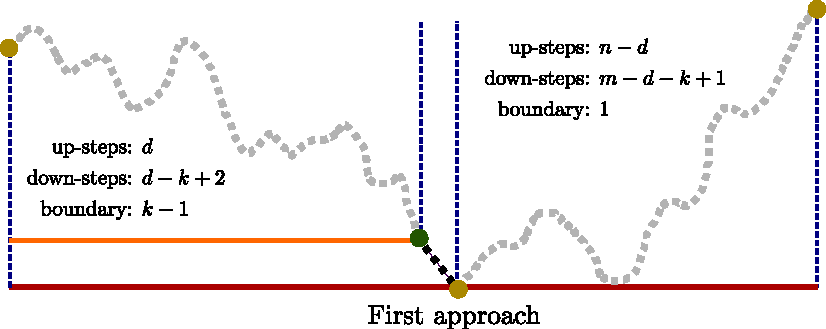
\includegraphics[width=\textwidth]{images/dyck_first_approach_sampling.pdf}
    \caption{Zooming into the error in Figure~\ref{fig:dyck_boundary_invariant}.
        We sample a position $x$ (yellow) on the boundary (red),
        such that the section of the path to the left of $x$ never approaches the red boundary (it respects the orange boundary).}
    \label{fig:dyck_mandatory_boundary_sampling}
\end{figure}

We will parameterize the position $x$ the number of up-steps $d$ between $x_i$ and $x$ (See Figure~\ref{fig:dyck_mandatory_boundary_sampling}).
implying that $x = x_{i} + 2d + k - 1$.
Given a specific $d$, we want to compute the number of valid paths that result in
$d$ up-steps before the first approach to the boundary.
Note that unlike Section~\ref{sec:sampling_the_height}, $d$ is used here to parameterize the (horizontal) $x$-position of the desired point.
We will calculate the probability $p_d$ associated with a particular position
by counting the total number of paths to the left and right of the first approach and multiplying them together.

As in Section~\ref{sec:the_difficult_case}, we define
$S_{left}$ to be the number of paths in the sub-interval before the first approach (left side of Figure~\ref{fig:dyck_mandatory_boundary_sampling}),
$S_{right}$ to be the number of paths following the first approach,
and $S_{total}$ to be the total number of paths that touch the ``mandatory boundary'' at $k$
(note that these quantities are functions of $U,D,k$ and $d$, but we drop the parameters for the sake of clarity):
{\small
\begin{align*}
    S_{left} = C_{k}(d, d+k-2)
    &&S_{right} = C_1(U-d, D-d-k+1)
    &&S_{total} = C_k(U,D) - C_{k-1}(U,D)
\end{align*}}
Our goal is to sample $d$ from the distribution $\{ p_d\}$ where $p_d = S_{left}\cdot S_{right}/S_{total}$.
The application of Lemma~\ref{lem:rejection_sampling} requires us to approximate $\{p_d\}$
with a ``well behaved'' $\{q_d\}$ (one whose CDF can be efficiently estimated).
Since we only require a asymptotic (up to $\poly(\log n)$ factors) approximation to $\{p_d\}$,
it suffices to estimate the number of paths asymptotically as well.
Using Equation~\ref{eq:catalan_trapezoid}, we obtain approximations for $S_{left}$ and $S_{right}$
(Lemma~\ref{lem:ReturnDLeftBound} and Lemma~\ref{lem:ReturnDRightBound} with proofs in Section~\ref{sec:omitted_supporting_first_return_queries}).
Our general strategy will be to integrate continuous versions of these approximations in order to obtain a CDF of some approximating distribution.
\begin{restatable}{lemma}{ReturnDLeftBound}
\label{lem:ReturnDLeftBound}
If $d > \log^4 n$, then $S_{left}(d)
= \Theta\left( \frac{2^{2d+k}}{\sqrt{d}}\mathlarger e^{-r_{left}(d)}\cdot \frac{k-1}{d+k-1}\right)$
where $r_{left}(d) = \frac{(k-2)^2}{2(2d+k-2)}$.
Furthermore, $r_{left}(d)=\mathcal O(\log^2 n)$.
\end{restatable}

\begin{restatable}{lemma}{ReturnDRightBound}
\label{lem:ReturnDRightBound}
If $U+D-2d-k > \log^4 n$, then $S_{right}(d)
= \Theta\left( \frac{2^{U+D-2d-k}}{\sqrt{U+d-2d-k}}\mathlarger e^{-r_{right}(d)}\cdot \frac{U-D+k}{U-d+1}\right)$
where $r_{right}(d) = \frac{(U-D-k-1)^2}{4(U+D-2d-k+1)}$.
Furthermore, $r_{right}(d)=\mathcal O(\log^2 n)$.
\end{restatable}

Unfortunately, these continuous approximation functions obtained do not admit closed form integrals.
The main culprit is the exponential term in both expressions.
We tackle this issue by noticing that the values of the exponents are bounded by $\mathcal O(\log^2 n)$ over the majority of the range of $d$.
Within this range of $d$ values, the approximating functions may be further simplified by taking a piecewise linear approximation,
where each of the pieces corresponds to a fixed value of the \emph{floor of the corresponding exponent}.
This technique is elaborated in Section~\ref{sec:estimating_the_cdf}.

We now consider the \emph{``problematic''} values of $d$ that are outside the range of the two preceding lemmas.
These values are the ones where $d < \log^4 n$ or $2d > U+D-k-\log^4 n$.
Since $d$ is the number of up steps in the left sub-interval, $d \ge 0$.
Further, since the length of the right sub-interval nust be non-negative (see Figure~\ref{fig:dyck_mandatory_boundary_sampling}),
we get $U+D-2d-k+1 \ge 0$.
Thus, we define the \emph{``problematic''} set:
\begin{align}
\label{eq:SetDefinition}
    \mathcal R = \left\{ d\ \mathlarger|\ 0\le d < \log^4 n \textrm{\textbf{\ or\ }} -1 < 2d-U-D+k < \log^4 n \right\}
\end{align}
Clearly, we can bound the size of this set as $|\mathcal R| = \mathcal O(\log^4 n)$.
An immediate consequence of Lemma~\ref{lem:ReturnDLeftBound} and Lemma~\ref{lem:ReturnDRightBound} is the following.

\begin{restatable}{corollary}{ReturnProbabilityBoundNotNormalized}
\label{cor:ReturnProbabilityBoundNotNormalized}
When $d\not \in \mathcal R$,
$S_{left}(d)\cdot S_{right}(d)
= \Theta\left( \frac{2^{U+D}}{\sqrt{d(U+D-2d-k)}}\cdot \mathlarger e^{-r(d)} \cdot \frac{k-1}{d+k-1}\cdot\frac{U-D+k}{U-d+1}\right)$
where $r(d)=\mathcal O(\log^2 n)$.
\end{restatable}



\subsubsection{Estimating the CDF}
\label{sec:estimating_the_cdf}
We use these observations to construct a suitable $\{q_d\}$ that can be used to invoke the rejection sampling lemma (Lemma~\ref{lem:rejection_sampling}).
We will achieve this by constructing a piecewise continuous function $\hat q$,
such that $\hat q(\delta)$ approximates $p_{\floor\delta}$, and then use the integral of $\hat q$ to define the discrete distribution $\{q_d\}$.
As stated in the previous section, we can leverage the fact that when $d \not \in \mathcal R$,
the floor of the exponent $\floor{r(d)}$ only takes $\mathcal O(\log^2 n)$ distinct values
(consequence of Corollary~\ref{cor:ReturnProbabilityBoundNotNormalized}).
Since the ``problematic'' set $\mathcal R$ only has $\mathcal O(\log^4 n)$ values,
we can also deal with these remaining values by simply creating $|\mathcal R|$ additional continuous pieces in the function $\hat q$.
We begin by rewriting $p_d = \Theta\left(\mathcal K \cdot f(d)\cdot e^{-r(d)}\right)$ where:
{\small
    \begin{align}
    \label{eq:dyck_integrable_function}
        \mathcal K = \frac{2^{U+D}}{S_{total}} = \frac{2^{U+D}}{C_k(U,D)-C_{k-1}(U,D)}\ \ \ \
        &&f(d) = \frac{(k-1)(U-D+k)}{\sqrt{d(U+D-2d-k)}(d+k-1)(U-d+1)}
    \end{align}}
Notice that $\mathcal K$ is a constant and $f(d)$ is a function whose integral has a closed form.
Using the fact that $r(d) = \mathcal O(\log^2 n)$ (Corollary~\ref{cor:ReturnProbabilityBoundNotNormalized}),
and $|\mathcal R| = \mathcal O(\log^4 n)$, we obtain the following lemma:

\begin{lemma}
\label{lem:ReturnProbabilityPiecewiseContinuous}
Given the piecewise continuous function
\begin{align*}
    \hat q(\delta) &=
    \begin{cases}
        p_{\floor\delta} &\mbox{if } \floor\delta \in \mathcal R \\ 
        \mathcal K\cdot f(\delta)\cdot exp\left(-\lfloor{r({\scriptstyle\floor\delta})}\rfloor\right)
        & \mbox{if } \floor\delta \not\in \mathcal R
    \end{cases}
    && \mathlarger \implies
    && p_d = \Theta\left( \int\limits_d^{d+1} \hat q(\delta)\right)
\end{align*}
Furthermore, $\hat q(\delta)$ has $\mathcal O(\log^4 n)$ continuous pieces.
%Note that this integral has a closed form for a fixed value of $\floor{r(d)}$.
\end{lemma}
\begin{proof}
For $d \in \mathcal R$, the integral trivially evaluates to exactly $p_d$.
For $d\not\in \mathcal R$, it suffices to show that $p_d = \Theta\left( \hat q(\delta)\right)$ for all $\delta\in [d,d+1)$.
We already know that $p_d = \Theta\left( \mathcal K\cdot f(d)\cdot e^{-r(d)}\right)$.
Moreover, for any $\delta\in [d,d+1)$, the exponential term $e^{-\floor{r(\floor\delta)}}$ in $\hat q(\delta)$
is within a factor of $e$ of the original $e^{-r(\floor\delta)}$ term.

For all $\mathcal O(\log^4 n)$ values $d\in \mathcal R$, $\hat q(\delta)$ is constant on the interval $[d,d+1]$.
Since $r(d) = \mathcal O(\log^2 n)$ by Corollary~\ref{cor:ReturnProbabilityBoundNotNormalized},
the exponential term $e^{-\floor{r(\floor\delta)}}$ in $\hat q(\delta)$ taken on at most $\mathcal O(\log^2 n)$ values.
Thus, $\hat q$ is continuous for a range of $\delta$ correspoding to a fixed value of $\floor{r(\floor\delta)}$,
and so, we conclude that $\hat q$ is piecewise continuous with $\mathcal O(\log^2 n)$ pieces.
\end{proof}

Now, we have everything in place to define the distribution $\{ q_d\}$ that we will be sampling from.
Specifically, we will define $q_d$ and it's CDF $Q_d$ as follows ($\mathcal N$ is the normalizing factor):
{\small
    \begin{align}
        q_d = \left(\int\limits_d^{d+1} \hat q(\delta)\right)\cdot \frac{1}{\mathcal N}
        && Q_d = \left(\int\limits_0^{d+1} \hat q(\delta)\right)\cdot \frac{1}{\mathcal N}
        && \textrm{where }\ \mathcal N = \int\limits_0^{d_{max}+1} \hat q(\delta)
    \end{align}}
%Here the normalizing factor $\mathcal N$ is $\int_0^{d_{max}+1} \hat q(\delta)$.
To show that these can be computed efficiently, it suffices to show that any integral of $\hat q(\delta)$ can be efficiently evaluated.
This follows from the fact that $\hat q$ is piecewise continuous with $\mathcal O(\log^4)$ pieces (Lemma~\ref{lem:ReturnProbabilityPiecewiseContinuous}),
each of which has a closed form integral (since $f(d)$ defined in Equation~\ref{eq:dyck_integrable_function} has an integral).

%However, we also need to be able to compute the constant $\mathcal K = 2^{U+D} = 2^{U+D}S_{total}$.
%The issue is that this value could be too large to compute.
%We mitigate this by fixing a threshold $\mathcal T = \Theta(\log^4 n)$, and ensuring that $U+D > \mathcal T$.
%In the case that $U+D \le \mathcal T$, we directly compute the $p_d$ values, and sample from the explicit distribution.
%Otherwise, we obtain the following lemma:}
%\begin{lemma}
%\label{lem:ReturnProbabilityConstant}
%If $U+D > \Theta(\log^4 n)$, the quantity $\mathcal K = 2^{U+D} = 2^{U+D}S_{total}$ is bounded \todo[inline]{finish}
%and can be computed efficiently.
%\end{lemma}
%\begin{proof}
%First, notice that $S_{total} = C_k(U,D) - C_{k-1}(U,D)$ is the number of paths with $U$ up steps and $D$ down steps with a boundary at $k$
%First, we compute a $\left( 1\pm 1/n^2\right)$ multiplicative approximation to $\log_2 S_{total}$,
%by using the strategy in Lemma~\ref{lem:probability_approximation_oracle} (Section~\ref{sec:computing_probabilities}).
%Now, we claim that 
%\end{proof}

\begin{lemma}
\label{lem:ReturnProbabilityPiecewiseContinuousIntegral}
Given the function $\hat q_d$ defined in Lemma~\ref{lem:ReturnProbabilityPiecewiseContinuous},
it is possible to approximate the integral $\int_{d_1}^{d_2+1} \hat q(\delta)$ to a multiplicative factor of $\left( 1\pm \frac{1}{n^2} \right)$,
in $\poly(\log n)$ time for any valid $d_1, d_2\in \mathbb Z$ (the bounds must be such that $d_i \ge 0$ and $U+D-2d_i-k+1 \ge 0$).
\end{lemma}
\begin{proof}
We will compute the integral by splitting it up into $\mathcal O(\log^4 n)$ continuous pieces and then approximating the integral over each piece.
The pieces corresponding to values of $\delta$ where $\floor\delta\in \mathcal R$
are explicitly computed as $p_d = \int\limits_d^{d+1} \hat q(\delta)$.
We can do this using Lemma~\ref{lem:probability_approximation_oracle} from Section~\ref{sec:computing_probabilities}.

Otherwise, if $\floor\delta\not\in \mathcal R$, we consider a range of values $[d_{min}, d_{max}]\subseteq [d_1, d_2+1]$,
such that for any $d\in [d_{min}, d_{max}]$, the value of $\floor{r(\floor{d})}$ is a constant $E$.
Recall that we can also compute a $\left( 1\pm 1/n^3\right)$ multiplicative approximation to $\ln \mathcal K = \ln 2\cdot(U + D) - \ln S_{total}$,
by using the strategy in Lemma~\ref{lem:probability_approximation_oracle} (Section~\ref{sec:computing_probabilities}).
Finally, we can compute $F = \int\limits_{d_{min}}^{d_{max}} f(\delta)$.
Now, the logarithm of the integral is be written as:
\[
\ln\left( \int\limits_{d_{min}}^{d_{max}} \hat q(\delta)\right) = \ln \left( \mathcal K\cdot E\cdot F\cdot\right)
= \ln 2\cdot(U + D) - \ln S_{total} + \ln E + \ln F
\]
If this value is smaller than $-3\ln n$, we can safely ignore it since it contrbuted less than $1/n^3$ to the probability mass.
On the flipside, the logarithm is guaranteed to be bounded by $\mathcal O(1)$.
The upper bound is a result of the fact that $\int \hat q(\delta) = \Theta(\sum p_d) = \mathcal O(1)$,
where both the sum and the integral are taken over the entire \emph{valid} range of $d$.
This means that we can exponentiate to obtain the true value of the piecewise integral up to a multiplicative approximation of $(1\pm 1/n^3)$.
Adding all the $\mathcal O(\log^4 n)$ pieces together produces the desired value of the integral.
\todo[inline,color=red!80!green!25]{Fix issues in this proof}
\end{proof}


Now, we are finally ready to use Lemma~\ref{lem:rejection_sampling} to sample $d$ from the distribution $\{p_d\}$,
using the efficient sampling procedure for $\{q_d\}$.
The only other requirement is the ability to approximate the $p_d$ values, which follows from Lemma~\ref{lem:probability_approximation_oracle}.
\begin{theorem}
\label{thm:first_return_in_interval}
Given a sub-interval $[x_{i},x_{i+1}]$ of a random Dyck path of length $2n$,
such that the only sampled heights in the interval are $y_i=\func{Height}(x_i)$ and $y_{i+1}=\func{Height}(x_{i+1})$,
and a mandatory boundary constraint at $k$,
there exists an algorithm that samples a point $x$ within the interval such that $\func{Height}(x) = y_i-k+1$,
using $\poly(\log n)$ time, random bits, and additional space.
\end{theorem}



\subsubsection{Finding the Correct Interval: $\func{First-Return}$ Query}
\label{sec:finding_the_correct_interval}
As before, consider all positions that have been queried already $ \langle x_1, x_2,\cdots, x_m \rangle$ (in increasing order)
along with their corresponding heights $ \langle y_1, y_2,\cdots, y_m \rangle$.
We wish to find the first return to height $y_i$ after $x_i$ (where $y_i = \func{Height}(x_i)$).
Our strategy begins by using Invariant~\ref{inv:boundary_invariant} to find the interval $\mathcal I = [x_k, x_{k+1}]$
containing $\func{First-Return}(x_i)$.
\begin{figure}[htpb]
    \centering
    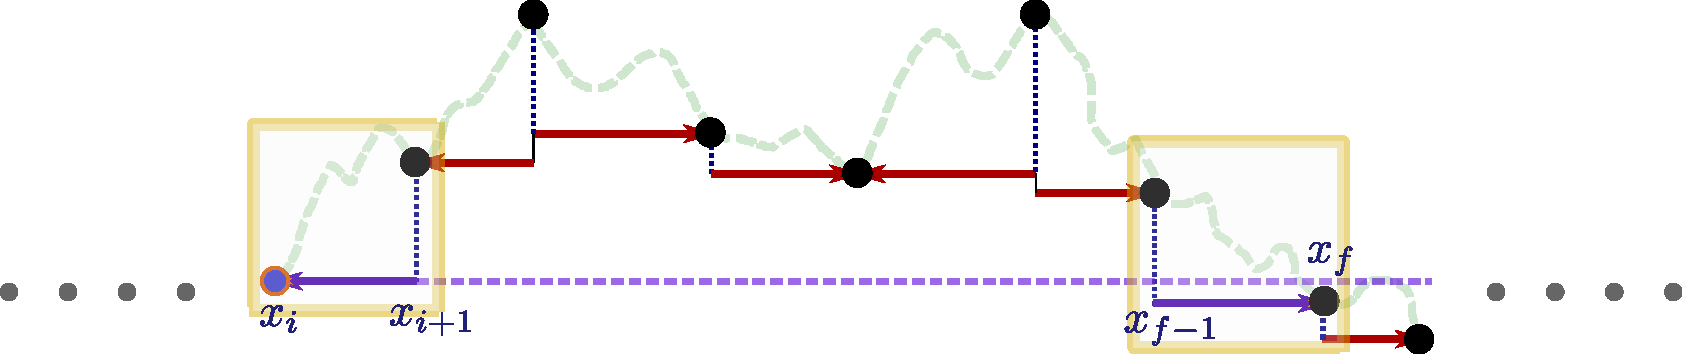
\includegraphics[width=\textwidth]{images/dyck_finding_correct_interval.pdf}
    \caption{There are only two possible intervals (yellow boxes) that could contain $\func{First-Return}(x_i)$;
    either the interval adjacent to $x_i$, or the interval $[x_{f-1}, x_f]$, where $f$ is the smallest index such that $y_f < x_i$.
    }
    \label{fig:dyck_finding_correct_interval}
\end{figure}
\begin{restatable}{lemma}{FirstReturnInterval}
\label{lem:first_return_interval}
For any position $x_i$, assuming that Invariant~\ref{inv:boundary_invariant} holds,
the interval $(x_{k-1},x_{k}]$ containing $\func{First-Return}(x_i)$ is obtained
by setting $k$ to be either the smallest index $f>i$ such that $y_f\le y_i$ or setting $k-1=i$.
\end{restatable}
\begin{proof}
We assume the contrary i.e. there exists some $k\not=f$ and $k\not=i+1$ such that the correct interval is $(x_{k-1},x_k]$.
Since $y_f<y_i$, the position of first return to $y_i$ happens in the range $(x_i,x_f]$.
So, the only possibility is $i+1 < k \le f-1$.
By the definition of $y_f$, we know that both $y_k$ and $y_{k-1}$ are strictly larger than $y_i$.
Invariant~\ref{inv:boundary_invariant} implies that the boundary for this interval $(y_{k-1},y_k]$ is at $\min(y_{k-1},y_k) > y_i$.
So, it is not possible for the first return to be in this interval.
\end{proof}

The good news is that there are only two intervals that we need to worry about, one of which is just the adjacent one $[x_i, x_{i+1}]$.
The problem of finding the other interval that may contain the first return boils down to finding the smallest index $f>i$ such that $y_f\le y_i$.
To this end, we define $M_{[a,b]}$ as the minimum sampled height in the range of positions $[a,b]$.
%(lowest $y$-value) of any sampled boundary in the range of positions $[a,b]$ along the Dyck path.

One solution is to maintain a range tree $\mathbf R$ \cite{comp_geo} over the range $[2n]$.
Assuming that $2n = 2^l$, we can view $\mathbf R$ as a complete binary tree with depth $r$.
Every non-leaf node is denoted by $\mathbf R_{[a,b]}$, and corresponds to a range $[a,b]\subseteq[2n]$ that is the union of the ranges of its children.
Each $\mathbf R_{[a,b]}$ stores the value $M_{[a,b]}$ which is is the minimum sampled height
in the range of positions $[a,b]$, or $\infty$ if none of the heights have been revealed.
%the height of the last boundary update that affected the entire range $[a,b]$.
The leaf nodes are denoted as $\{\mathbf R_i\}_{i\in[2n]}$, and correspond to the singleton range corresponding to position $i\in [2n]$.
%and by definition, this is the min of the values stored at the children of $\mathbf R_{[a,b]}$.
Note that a node at depth $l'$ will correspond to a range of size $2^{l-l'}$, with the root being associated with the entire range $[2n]$.

We say that the range $[a,b]$ is \emph{canonical} if it corresponds to a range of some $\mathbf{R}_{[a,b]}$ in $\mathbf R$.
By the property of range trees, any arbitrary range can be decomposed into a disjoint union of $O(\log n)$ canonical ranges.
We implement $\mathbf{R}$ to support the following operations:
\begin{itemize}
    \item \func{Update}$(x,y)$: Update the height of the position $x$ to $y$.\\
    This update affects all ranges $[a_i,b_i]$ containing $x$.
    So, for each $[a_i,b_i]$ we set $M_{[a_i,b_i]} = \min\left( M_{[a_i,b_i]}, y\right)$.
    \item \func{Query}$(a,b)$: Return the minimum boundary height in the range $[a,b]$.\\
    We decompose $[a,b]$ into $\mathcal O(\log n)$ \emph{canonical} ranges $ \langle r_1, r_2,\cdots\rangle$,
    %For each $r_i$, we compute $M_{r_i}$ as the minimum over all $R_r$ such that the \emph{canonical} range $r$ contains $r_i$.
    %Equivalently, we set $M_{r_i}$ to be the minimum of all values on the path from $\mathbf R_{r_i}$ to the root of $\mathbf R$,
    %which takes $\mathcal O(\log n)$ time.
    %Note that the values stores in the sub-tree rooted at $\mathbf R_{r_i}$ do not affect $M_{r_i}$,
    %since the coreesponding boundary updates did not affect the \emph{entire} range $r_i$ (these updates only affected canonical sub-ranges of $r_i$).
    and return the minimum of all the $M_{r_i}$ values as $M_{[a,b]}$ (since $[a,b]$ is the union of all $r_i$).
\end{itemize}

Now, we can binary search for $f$ by guessing a value $f'$ and checking if $\func{Query}(x_i,x_{f'}) \le y_i$.
Overall, this requires $\mathcal O(\log n)$ calls to $\func{Query}$, each of which makes $\mathcal O(\log n)$ probes to the range tree.
To avoid an initialization overhead, we only create the node $\mathbf{R}_{[a,b]}$ during the first $\func{Update}$ affecting a position $x\in[a,b]$.
Since a call to $\func{Update}$ can create at most $\mathcal O(\log n)$ new nodes in $\mathbf R$,
the additional space required for each $\func{Height}$ or $\func{First-Return}$ query is still bounded.

\begin{theorem}
\label{thm:dyck_first_return_sampling}
There is an algorithm using $\mathcal O(\log^{\mathcal O(1)} n)$ resources per query that provides access to a random Dyck path of length $2n$,
by answering queries of the form \func{First-Return}$(x_i)$ with the correctly sampled position $x'$;
where $x'>x_i$ is the position where the Dyck path first returns to $\func{Height}(x_i)$ after position $x_i$.
\end{theorem}
\begin{proof}
In order to make the presentation simpler, we ensure that the next determined position after $x_i$ is $x_i+1$ (i.e. $x_{i+1} = x_i + 1$).
This can be done by invoking $\func{Height}(x_i+1)$, if it has not been sampled already.
If $\func{Height}(x_i+1) = y_{i+1} < y_i$, we can terminate because $\func{First-Return}(x_i)$ is not defined.
Otherwise, we notice that in this setting, the first return cannot lie in the adjacent interval $[x_i,x_{i+1}] = [x_i, x_i+1]$.

Hence, we proceed to finding the smallest value $f$ such that $y_f < y_i$, by using the range tree data structure described above.
Since $\func{Height}(x_{f-1}) \ge y_i > \func{Height}(x_f)$ by definition, the interval $(x_{f-1},x_f]$ must contain a position at height $y_i$.
We sample a point in the middle of this interval and fix the boundary invariant by sampling another point,
essentially breaking it up into $\mathcal O(1)$ sub-intervals each at most half the size of the original.
Based on the new samples, we again find the (newly created) sub-interval containing the first return in $\mathcal O(1)$ time.
We repeat up to $\mathcal O(\log n)$ times, performing binary search to find the position of the first return.
%\todo{Remove Threshold}
%We repeat up to $\mathcal O(\log n)$ times until the current interval size drops below the threshold $\mathcal T$.
%Then we spend $\widetilde{\mathcal O}(\mathcal T)$ time to brute force sample this interval and find the first return position (if it wasn't revealed in previous steps).
\end{proof}

\subsubsection{Maintaining \func{Height} Queries under Invariant~\ref{inv:boundary_invariant}}
\label{sec:maintaining_height_queries_under_invariant}
Finally, we show that the boundary constraints introduced in order to maintain Invariant~\ref{inv:boundary_invariant}
do not interfere with the implementation of \func{Height} queries.
As before, we consider the currently revealed heights $ \langle y_1, y_2,\cdots, y_m \rangle$,
along with the corresponding positions $ \langle x_1, x_2,\cdots, x_m \rangle$ (in increasing order).
Say that we are now presented with a a query $\func{Height}(x)$, where $x_i < x < x_{i+1}$.
As in Section~\ref{sec:sampling_the_height}, we swap $x_i$ and $x_{i+1}$ if necessary in order to ensure that $y_i < y_{i+1}$.
Due to Invariant~\ref{inv:boundary_invariant}, we know that the lowest achievable height in the interval $[x_i, x_{i+1}]$ is $y_i$,
i.e. the boundary constraint for the left half becomes $k = 1$ instead of $k = y_i + 1$, since the constrained boundary is at height $y_i$.
Similarly, the boundary constraint for the right half becomes $k' = 2U - 2D + 1$.
The rest of the algorithm can proceed as described in Section~\ref{sec:sampling_the_height}.
Of course, in this scenario, the boundary is never far away, and therefore we should always use the strategy in Section~\ref{sec:the_difficult_case}.
This allows us to combine the results from Theorem~\ref{thm:dyck_height_sampling} and Theorem~\ref{thm:dyck_first_return_sampling},
thus obtaining the following implementation
\CatalanGrand*


\subsection{\func{Reverse-First-Return} Queries}
\label{sec:reverse_first_return_queries}
\todo[inline,color=red!80!green!25]{Write this}
